
\documentclass[conference]{IEEEtran}

\usepackage[spanish]{babel}
\usepackage{amsmath,amssymb,amsfonts,amsthm}
\usepackage{graphicx}
%\usepackage{bbm}
\usepackage[utf8]{inputenc} % Caracteres en Español (Acentos, ñs)
\usepackage{url} % ACENTOS
\usepackage{hyperref} % Referencias
\usepackage{subfig}
\usepackage{lipsum}
\usepackage{balance}


\usepackage{geometry}
\usepackage{graphicx}
\usepackage{adjustbox}



%%%%%%%%%%%%%%%%%%%%%%%%%%%%%%%%%%%%%%%%%%%%%
% PARCHE PARA ELIMINAR LA FECHA DEL DOCUMENTO
% 
\usepackage{etoolbox}
\makeatletter
% \frontmatter@RRAP@format is responsible for the parentheses
\patchcmd{\frontmatter@RRAP@format}{(}{}{}{}
\patchcmd{\frontmatter@RRAP@format}{)}{}{}{}
%\renewcommand\Dated@name{}
\makeatother	
% FIN DEL PARCHE
% 
%%%%%%%%%%%%%%%%%%%%%%%%%%%%%%%%%%%%%%%%%%%%%

%%%%%%%%%%%%%%%%%%%%%%%%%%%%%%%%%%%%%%%%%%%%%
% PARCHE PARA PERMIRIR UTILIZAR BIBLATEX EN ESTA PANTLLA
%\PassOptionsToPackage{square,numbers}{natbib}
%\RequirePackage{natbib}  
%%%%%%%%%%%%%%%%%%%%%%%%%%%%%%%%%%%%%%%%%%%%%

\usepackage[backend=bibtex,sorting=none]{biblatex}
% Estas lineas permiten romper los hipervinculos muy largos !!!!
\setcounter{biburllcpenalty}{7000}
\setcounter{biburlucpenalty}{8000}
\addbibresource{references.bib}

% Actualiza en automático la fecha de las citas de internet a la fecha de la compilación del documento
\usepackage{datetime}
\newdateformat{specialdate}{\twodigit{\THEDAY}-\twodigit{\THEMONTH}-\THEYEAR}
\date{\specialdate\today}

% la sentencia \burl en las citas... 
\usepackage[hyphenbreaks]{breakurl}

\renewcommand\spanishtablename{Tabla}
\renewcommand\spanishfigurename{Figura}

%\usepackage{datetime}
%\newdateformat{specialdate}{\twodigit{\THEDAY}-\twodigit{\THEMONTH}-\THEYEAR}
%\newdateformat{specialdate}{\twodigit{\THEDAY}-\THEYEAR}
%\date{\specialdate\today}


\begin{document}
%%%%%%%%%%%%%%%%%%%%%%%%%%%%%%%%%%%%%%%%%%%%%
% Definitions
%
%
% Define your special symbols here
%
%%%%%%%%%%%%%%%%%%%%%%%%%%%%%%%%%%%%%%%%%%%%%

% use to set width of figures
\newcommand{\breite}{0.9} %  for twocolumn
\newcommand{\RelacionFiguradoscolumnas}{0.9}
\newcommand{\RelacionFiguradoscolumnasPuntoCinco}{0.45}


%%%%%%%%%%%%%%%%%%%%%%%%%%%%%%%%%%%%%%%%%%%%%
% End Definitions
%%%%%%%%%%%%%%%%%%%%%%%%%%%%%%%%%%%%%%%%%%%%%


%Title of paper
\title{Reporte de Proyecto de Equipo \\ 
Lenguaje de Señas Mexicano}

% Trabajo Individual
\author{\IEEEauthorblockN{Osiel Alejandro Ordoñez Cruz\IEEEauthorrefmark{1}, César Aldahir Flores Gámez\IEEEauthorrefmark{1}, \\Daniel Eduardo Macias Estrada\IEEEauthorrefmark{1}, Lorena Marisol Romero Hernández\IEEEauthorrefmark{1}, \\Mauricio Hernández Cepeda\IEEEauthorrefmark{1}}
% En caso de trabajos en equipo, poner a todos los autores en estricto ORDEN ALFABETICO
%\author{\IEEEauthorblockN{Michael Shell\IEEEauthorrefmark{1},
%Homer Simpson\IEEEauthorrefmark{1},
%James Kirk\IEEEauthorrefmark{1}, 
%Montgomery Scott\IEEEauthorrefmark{1} and
%Eldon Tyrell\IEEEauthorrefmark{1}}
\IEEEauthorblockA{\IEEEauthorrefmark{1}Ingeniería en Tecnologías de la Información\\
Universidad Politécnica de Victoria}
}


%\date{}

\maketitle

\begin{abstract} 

El presente reporte tiene como objetivo explicar sencilla y detalladamente la continuación del desarrollo de una aplicación con GUI en la que se logra el entrenamiento, aprendizaje e interpretación del Lenguaje de Señas Mexicano (LSM), utilizando Python como lenguaje de desarollo, además de diversas librerías usadas en sistemas inteligentes, así como OpenCV para la visión artificial, de tal manera que se comprenda la manera en que se realiza el entrenamiento y como el algortimo interpreta las señas usando los datasets generados a partir del entrenamiento previo.

\end{abstract}


%\maketitle must follow title, authors, abstract, \pacs, and \keywords




\section{Introducción}

A lo largo del seguimiento del proyecto, se comprendió y en ocasiones se modificó una serie de programas con el objetivo de mejorar una aplicación la cual cuenta con interfaz gráfica y presentar al usuario una aplicación que sea capaz de detectar y comprender el \textbf{Lenguaje de Señas Mexicano (LSM)} \cite{simonyan2014very}.

Dicha aplicación esta desarrollada en \textbf{Python} \cite{goodfellow2016deep} \cite{he2016deep}, con este, se empleó el paradigma de la Programación Modular, debido a que se hizo más sencillo la codificación de funciones específicas de aprendizaje, las cuales pudieran ser reutilizadas en otras secciones del programa.

Para la generación de los elementos gráficos se implementó como principal librería \textbf{OpenCV} \cite{opencv_library} \cite{wu2018group}, por otro lado se utilizaron otras librerías ampliamente conocidas en el área de Sistemas Inteligentes como lo es \textbf{numpy} \cite{lecun2015deep} para el manejo de datos númericos en conjunto con \textbf{pandas} \cite{szegedy2015going} y \textbf{matplotlib} \cite{kingma2014adam} por el lado del entrenamiento, además de \textbf{sklearn} \cite{liu2016ssd} para la carga de datos, y por supuesto, la tan utilizada \textbf{tensorflow} \cite{abadi2016tensorflow} para el entrenamiento de la red neuronal.




\section{Desarrollo Experimental}

En el contexto del desarrollo tecnológico, se cuenta con un proyecto previo desarrollado por colegas de la carrera de Tecnologías de la Información. Dicho proyecto consiste en la detección de señas en \textbf{Lenguaje de Señas Mexicano (LSM)}, logrando identificar exitosamente alrededor de 30 gestos. A partir de este punto, se plantea la iniciativa de expandir el algoritmo previamente construido en \textbf{OpenCV}, con el propósito de entrenar y reconocer un 30\% adicional de estas señas.

Previo al inicio del desarrollo de este nuevo proyecto, es esencial tener en cuenta ciertos antecedentes fundamentales.

\textbf{Antecedentes sobre el Lenguaje de Señas Mexicano (LSM):}
\begin{itemize}
    \item El Lenguaje de Señas Mexicano (LSM) representa un sistema de comunicación gestual utilizado por la comunidad de personas sordas en México. Su función radica en la expresión de ideas, pensamientos y emociones. Siguiendo la misma línea que otros lenguajes de señas en el mundo, el LSM se basa en el empleo de gestos y movimientos manuales, así como en las expresiones faciales y corporales, para transmitir información de forma visual, en contraposición al medio auditivo.
\end{itemize}


\textbf{Elementos Esenciales del Lenguaje de Señas Mexicano:}
El LSM está compuesto por diversos componentes que se combinan para otorgarle su riqueza y capacidad expresiva:
\begin{itemize}
    \item \textbf{Signos Manuales: }Corresponden a gestos ejecutados con las manos y dedos, encargados de representar palabras, conceptos e ideas. Cada signo tiene una significado específico, pudiendo estar conformado por la posición de las manos, los movimientos y su localización en relación al cuerpo.

    \item \textbf{Expresiones Faciales:} Estas son de vital importancia en el LSM, ya que a menudo definen la gramática y matices de una oración. Cambios en cejas, ojos y boca pueden indicar diversas emociones, tonos y contextos.

    \item \textbf{Movimientos Corporales:} En conjunto con los signos y expresiones faciales, los movimientos corporales, como inclinación de la cabeza, hombros y cuerpo, añaden información suplementaria a la comunicación en LSM.

    \item \textbf{Espacio y Dirección: }El espacio alrededor del cuerpo se aprovecha para señalar la ubicación de objetos y personas. Movimientos de las manos hacia distintas áreas del espacio pueden representar lugares y personas específicas.
    
\end{itemize}

\textbf{Consideraciones para la Implementación de LSM en OpenCV:}
Si se aspira a llevar a cabo un programa en OpenCV que facilite la comunicación en Lenguaje de Señas Mexicano, es crucial tener en mente los siguientes aspectos:
\begin{itemize}
    \item \textbf{Diseño de la Interfaz Gráfica:} Aprovechar las capacidades de diseño de OpenCV para crear una interfaz gráfica intuitiva y de fácil uso. Se pueden emplear botones o áreas de dibujo para permitir a los usuarios ejecutar los signos manuales y las expresiones faciales correspondientes.

    \item \textbf{Captura de Gestos:} Implementar un mecanismo que registre los gestos realizados por el usuario. Esto podría abarcar el seguimiento en tiempo real de las posiciones de las manos y dedos.

    \item \textbf{Reconocimiento de Signos:} Idear un sistema que sea capaz de reconocer los signos manuales introducidos por el usuario. Algoritmos de reconocimiento de patrones pueden emplearse para identificar gestos y asociarlos a las palabras o conceptos pertinentes.

    \item \textbf{Animaciones y Expresiones Faciales:} Introducir la posibilidad de modificar las expresiones faciales en la interfaz gráfica. Esto podría involucrar el uso de imágenes o animaciones que representen diversas emociones y estados.

    \item \textbf{Feedback Visual:} Proporcionar retroalimentación visual a medida que los usuarios interactúan con la interfaz. Esto podría comprender la visualización de gestos efectuados, la representación de signos manuales en formato de texto y la adaptación de expresiones faciales según la comunicación.
    
\end{itemize}

\textbf{Proceso de Reentrenamiento del Sistema de Lenguaje de Señas}

\begin{enumerate}
    \item \textbf{Preparación de Carpetas y Definición de Señas:} En primera instancia, se establece la estructura de carpetas para almacenar los datos. Las señas que se capturarán se organizan en las siguientes rutas: $"dataset\_generator/original\_dataset/data"$, $"dataset\_generator/original\_dataset/Face"$, $"dataset\_generator/original\_dataset/Hands" $y $"dataset\_generator/original\_dataset/Torso"$.

    Luego, se procede a ejecutar el archivo $"txtextracter.py"$ ubicado en la carpeta de módulos. Este archivo desempeña un rol fundamental al definir las señas que serán capturadas. En específico, se ingresan las señas en los arreglos $"word\_bank"$ y $"word\_list"$.

    \item \textbf{Extracción de Datos en Tiempo Real:} Una vez configuradas las señas, se inicia el proceso de captura de datos en tiempo real. Para ello, se ejecuta el script correspondiente, el cual hace uso de la función $"live\_data\_extracter"$. Mediante el módulo Holistic de MediaPipe, se detectan puntos de referencia en las manos, el rostro y el cuerpo a partir de la cámara web. Cada señal se registra diez veces, con un avance al presionar la tecla 'a'. Los datos extraídos se almacenan en archivos CSV.

    \item \textbf{Procesamiento y Almacenamiento de Datos:} Con los datos capturados en CSV, se procede a ejecutar el archivo $"dataExtracter.py"$ dentro de la carpeta de módulos. Este archivo se encarga de leer los archivos CSV con información de las coordenadas de puntos de referencia en las manos. Los datos se procesan para calcular distancias y ángulos, generando nuevas estructuras de datos. Los resultados se almacenan en carpetas adecuadamente estructuradas en la ruta $"../../original\_dataset/data"$.

    \item \textbf{Generación del Dataset y Entrenamiento del Modelo:} El siguiente paso implica la ejecución del archivo $"main.py"$ ubicado en la carpeta $"code"$. En este punto, se debe seleccionar la opción $"1"$ para generar el dataset en base a los archivos CSV recopilados y procesados.

    Una vez completada la generación del dataset, se elige la opción $"2"$. Aquí, se lleva a cabo el entrenamiento del modelo y las etiquetas de las clases. Los resultados de este proceso se almacenan como $"best\_model.h5"$ y $"le\_name\_mapping.txt"$ en la carpeta $"dataset\_generator"$. Estos archivos reemplazarán a los existentes en la carpeta principal del LSM, denominada $"desktop\_app"$.

    
    Es importante remarcar que para el correcto funcionamiento, se debe adaptar el contenido del archivo $"le\_name\_mapping.txt"$ antes de su reemplazo. Esto involucra el cambio de comillas simples por dobles y el encapsulamiento de los números con comillas dobles, a fin de que estos archivos sean interpretados correctamente como formato JSON
\end{enumerate}

\textbf{Proceso de Evaluación del Modelo Post-Entrenamiento}

\begin{itemize}
    \item En el código, para realizar la evaluación se hace uso tanto de $x\_train$ como $y\_train$ los cuales se cargan con los datos del directorio $../dataset$, y lo mismo sucede con $x\_test$ y $y\_test$. Sin embargo, esto no divide explícitamente los datos en conjuntos de entrenamiento y prueba.
    \item Para lograr lo anterior, se utiliza el argumento $validation\_split$ en la función $model.fit()$ con el propósito de especificar el porcentaje que se utilizará como conjunto de validación durante el entrenamiento.
    \item Para ello, $validation\_split$ se le otorga un valor de $0.2$ ($validation\_split=0.2$), lo que significa que el $20\%$ de los datos de entrenamiento se utilizarán como conjunto de validación durante el entrenamiento, y el $80\%$ restante se utlizará para el entrenamiento real del modelo.
    \item En resumen, el $80\%$ de los datos se usan para el entrenamiento, el $20\%$ se utilizan como conjunto de validación durante el entrenamiento, y los datos en $x\_test$ y $y\_test$ son usados para la evaluación final del model después del entrenamiento.
\end{itemize}

\begin{figure}[h]
\centering
{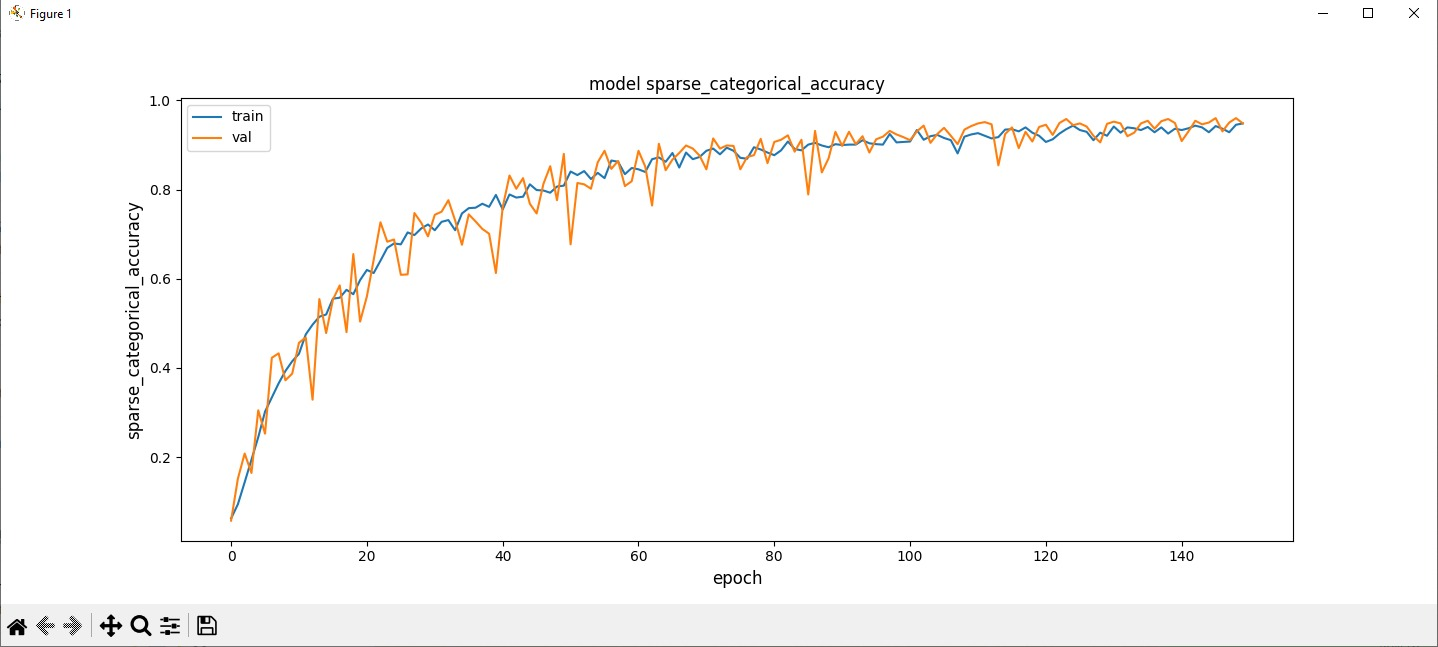
\includegraphics[width=0.95\linewidth]{img/grafica-evaluacion-de-modelo.jpeg}}
\caption{Gráfica de Evaluación del Modelo}
\label{fig:1}
\end{figure}

\section{Resultados}
En la etapa de resultados, se enfoca en capturar las señas mediante la cámara y procesar los datos para su posterior entrenamiento, lo que constituye un paso crucial en la mejora y reentrenamiento del Sistema de Lenguaje de Señas Mexicano, figura \ref{fig:1}.


\begin{figure}[h]
\centering
{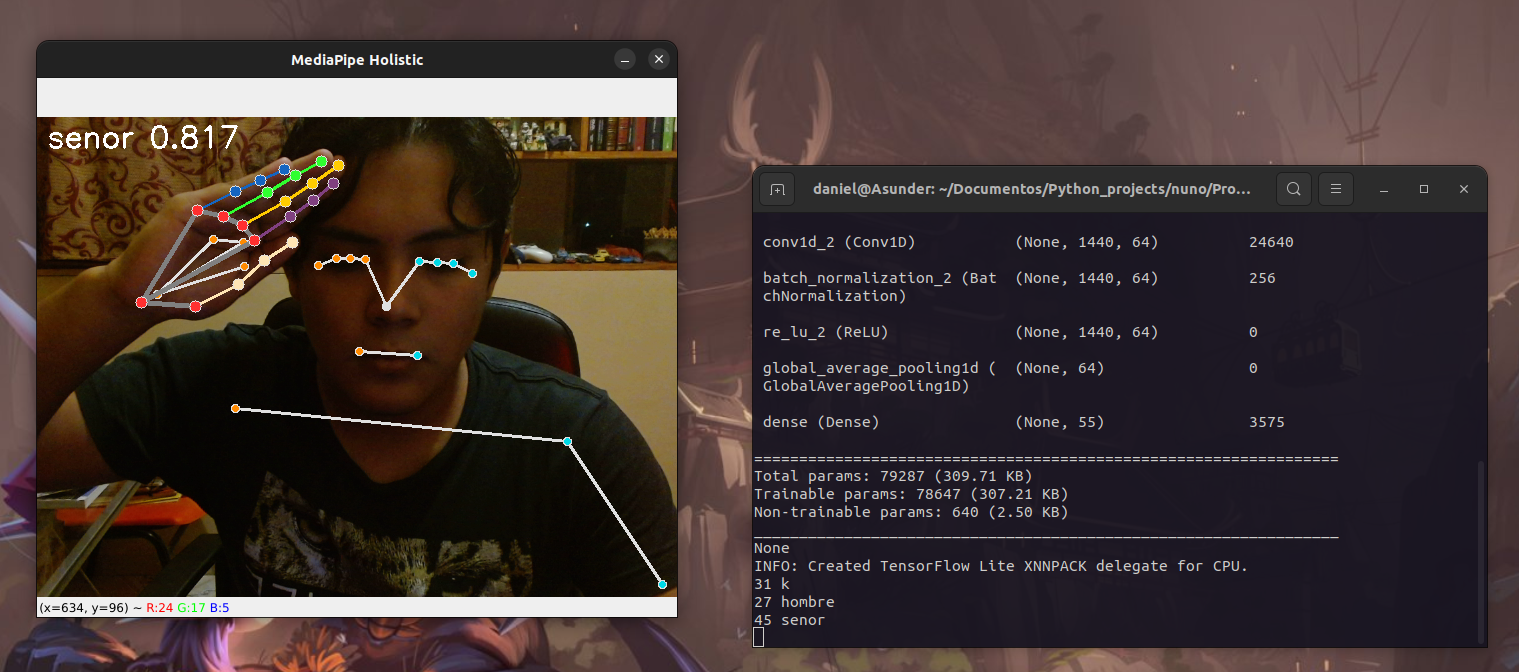
\includegraphics[width=0.95\linewidth]{img/01.png}}
\caption{Ejecución del programa; seña de la palabra "señor"}
\label{fig:1}
\end{figure}

Después de la generación del dataset y el entrenamiento del modelo, se procede a evaluar su rendimiento. Esta etapa es esencial para determinar la efectividad del sistema en la interpretación de las señas capturadas. La evaluación del modelo puede involucrar técnicas como la validación cruzada o la división del dataset en conjuntos de entrenamiento y prueba, figura  \ref{fig:2}.


\begin{figure}[h]
\centering
{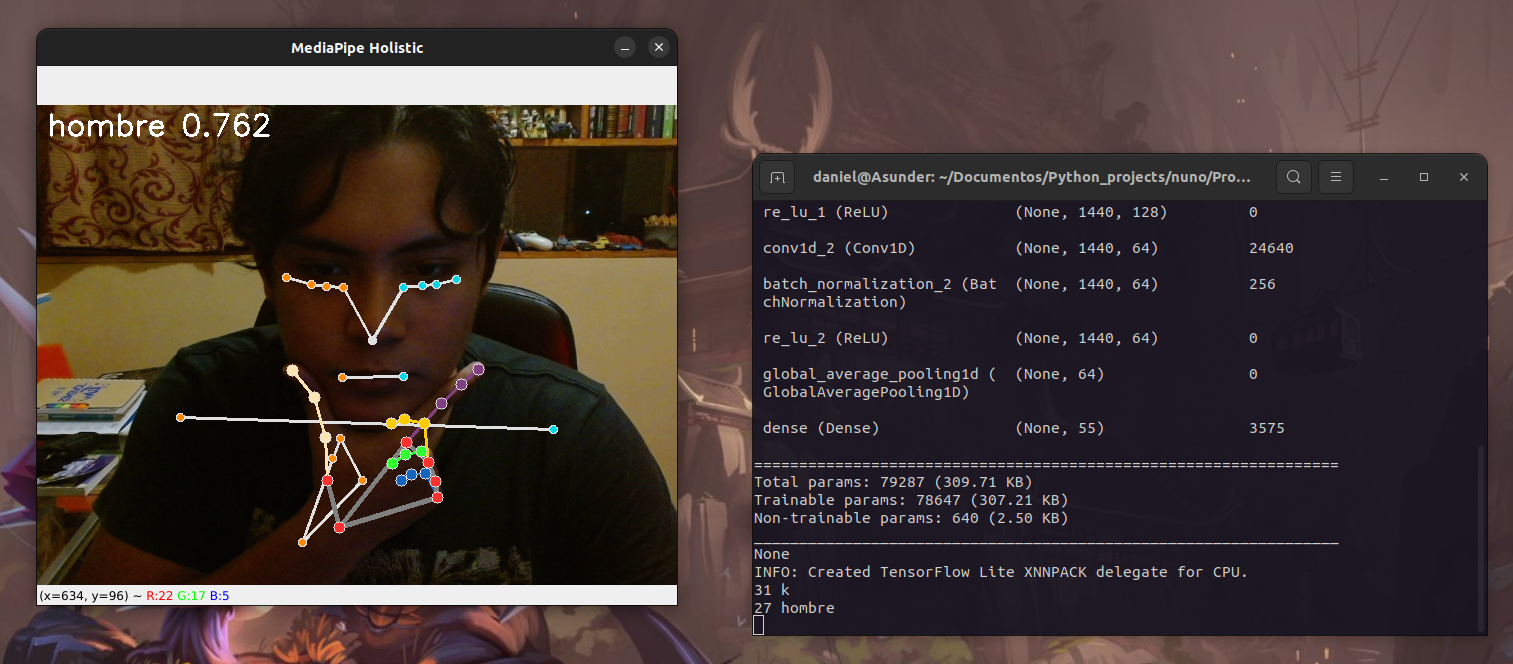
\includegraphics[width=0.95\linewidth]{img/02.png}}
\caption{Seña de la palabra "hombre"}
\label{fig:2}
\end{figure}

En esta fase, se utilizan las señas capturadas en la cámara para verificar cómo el modelo interpreta y reconoce estas señas en tiempo real. Esto puede incluir la interfaz del LSM en la que los usuarios realizan las señas y el sistema responde adecuadamente, figura \ref{fig:3}.



\begin{figure}[h]
\centering
{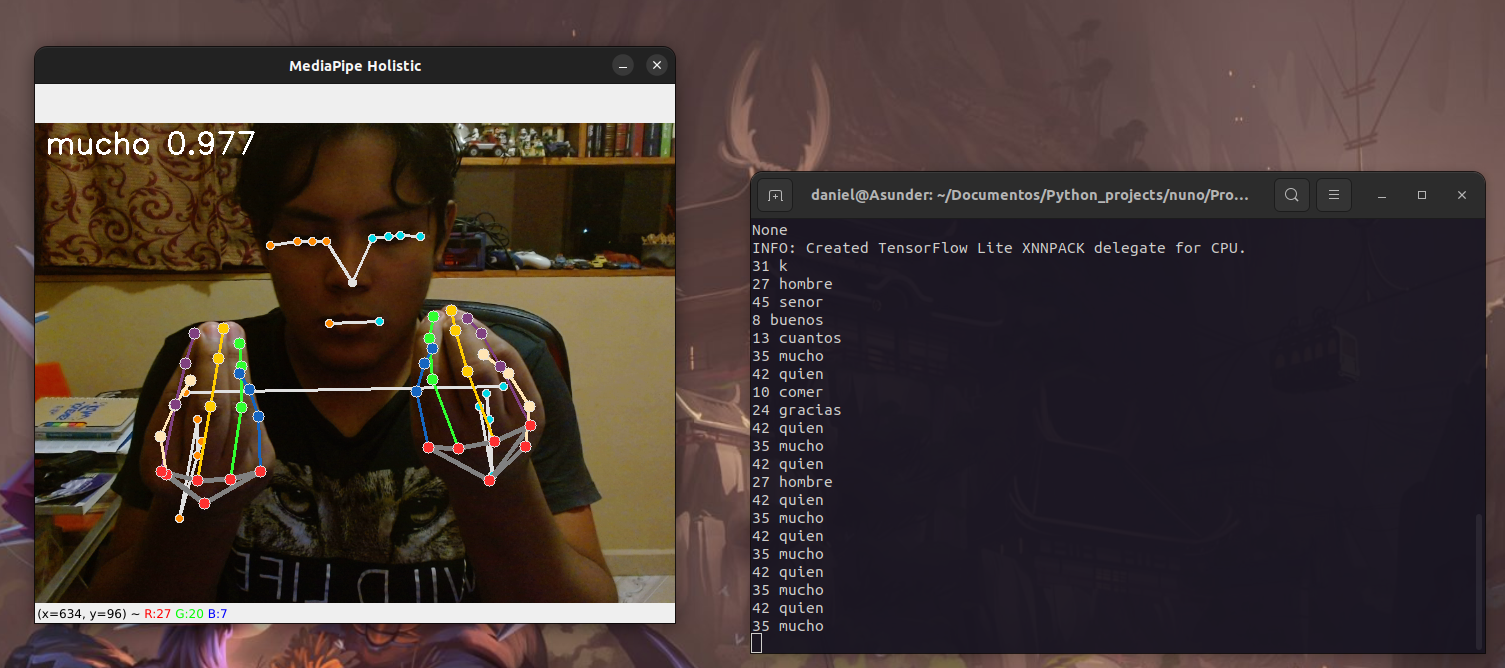
\includegraphics[width=0.95\linewidth]{img/03.png}}
\caption{Seña de la palabra "muchos"}
\label{fig:3}
\end{figure}

La etapa de resultados en el proceso de reentrenamiento del Sistema de Lenguaje de Señas Mexicano abarca desde la generación del dataset hasta la evaluación del modelo, ajustes, pruebas en tiempo real y mejoras continuas. Este proceso garantiza que el sistema sea capaz de interpretar con precisión las señas capturadas en la cámara y proporcionar una herramienta efectiva para la comunicación en lenguaje de señas mexicano, figura \ref{fig:4}. A continuación se pueden observar el resto de pruebas que se realizaron en la figura \ref{fig:5}, \ref{fig:6}, \ref{fig:7}, \ref{fig:8}, \ref{fig:9}

\begin{figure}[h]
\centering
{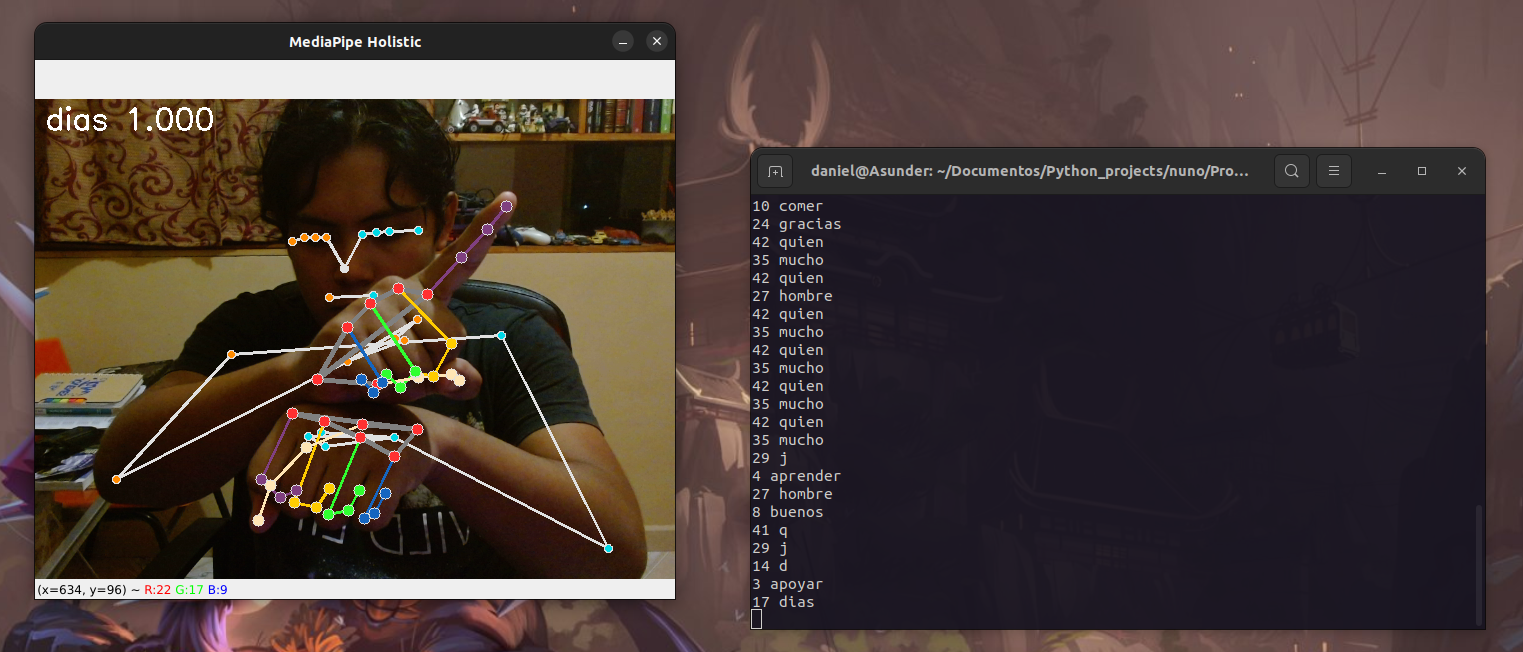
\includegraphics[width=0.95\linewidth]{img/04.png}}
\caption{Seña de la expresión "Buenos días"}
\label{fig:4}
\end{figure}

\begin{figure}[h]
\centering
{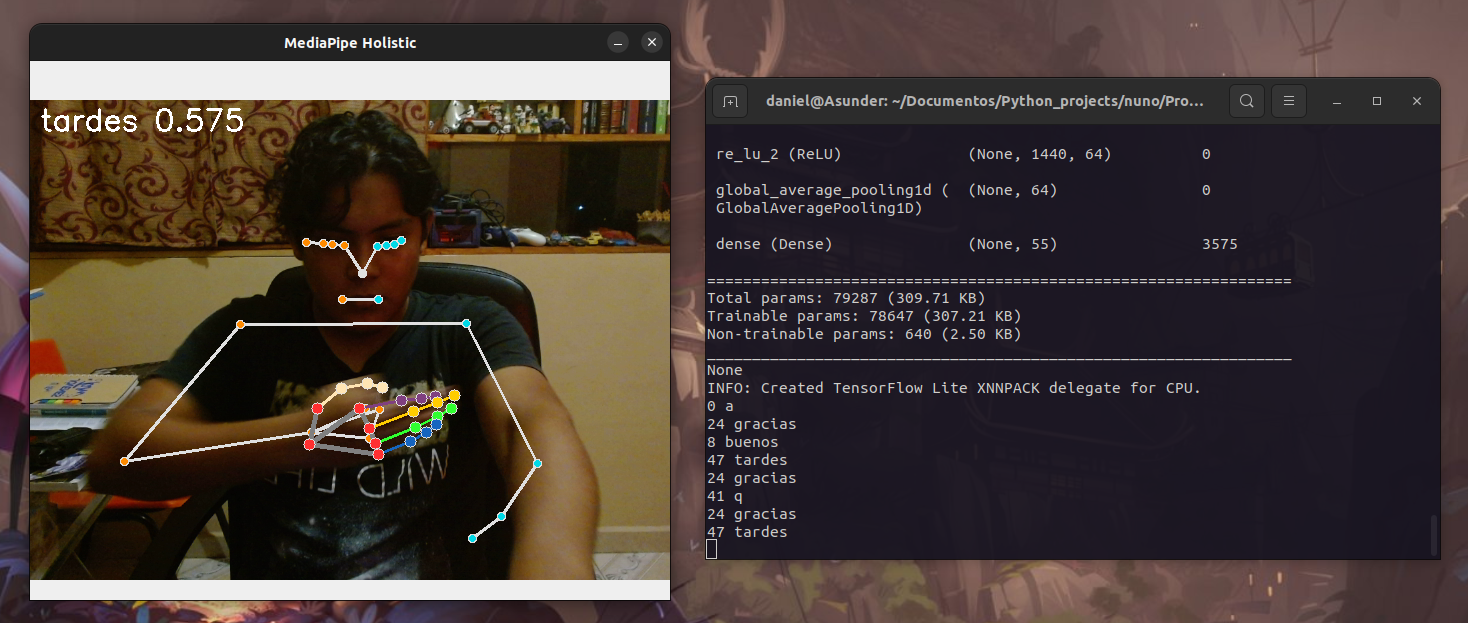
\includegraphics[width=0.95\linewidth]{img/05.png}}
\caption{Seña de la expresión "Buenas tardes"}
\label{fig:5}
\end{figure}

\begin{figure}[h]
\centering
{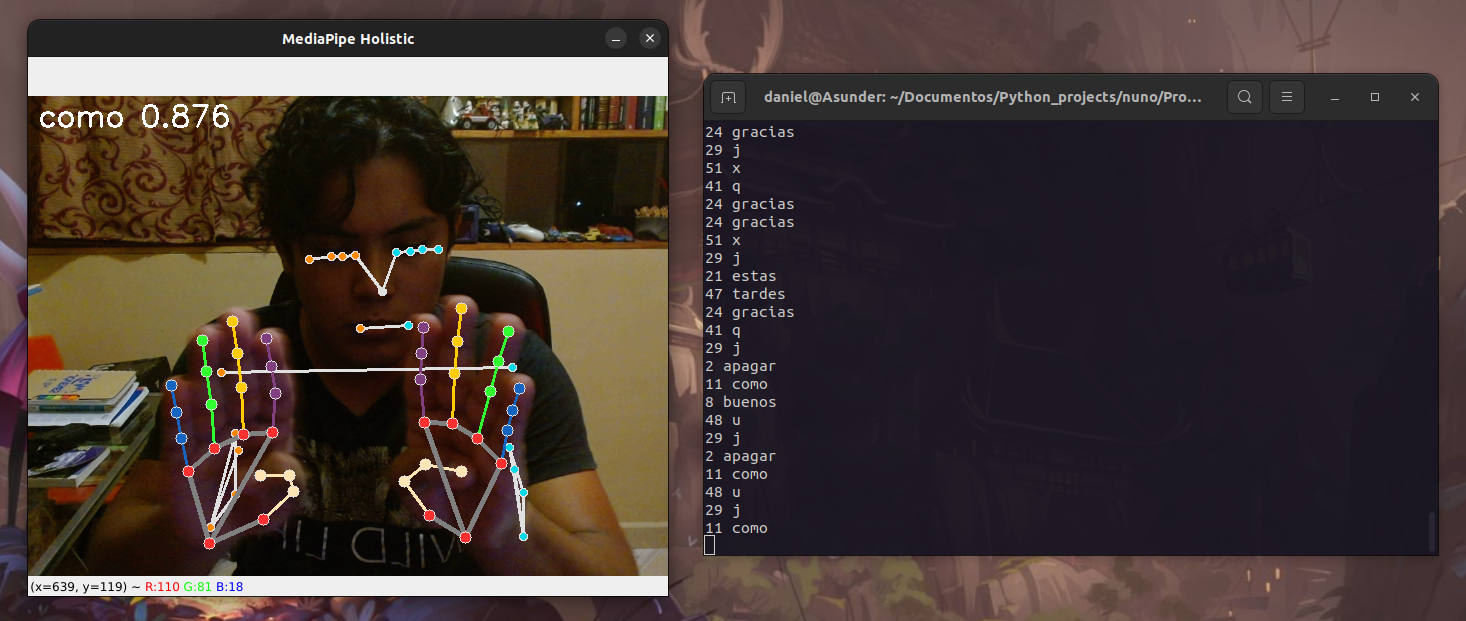
\includegraphics[width=0.95\linewidth]{img/06.png}}
\caption{Seña de la palabra "¿Cómo?"}
\label{fig:6}
\end{figure}

\begin{figure}[h]
\centering
{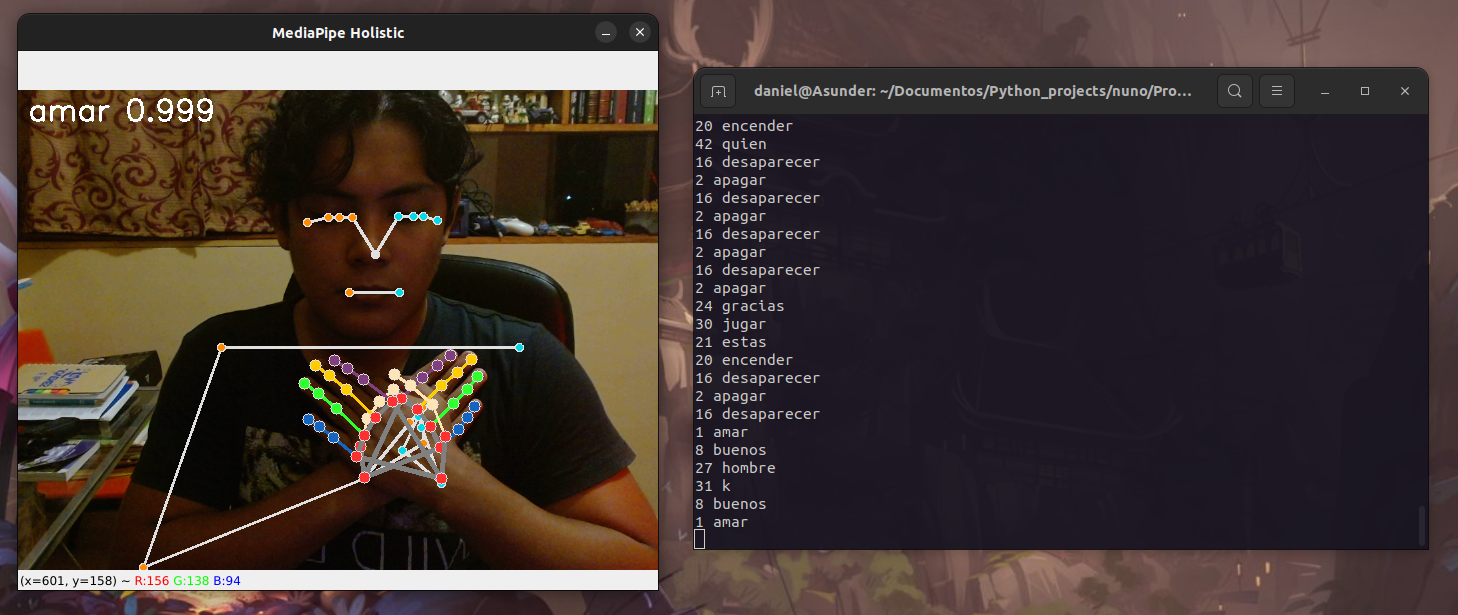
\includegraphics[width=0.95\linewidth]{img/07.png}}
\caption{Seña de la palabra "amor"}
\label{fig:7}
\end{figure}

\begin{figure}[h]
\centering
{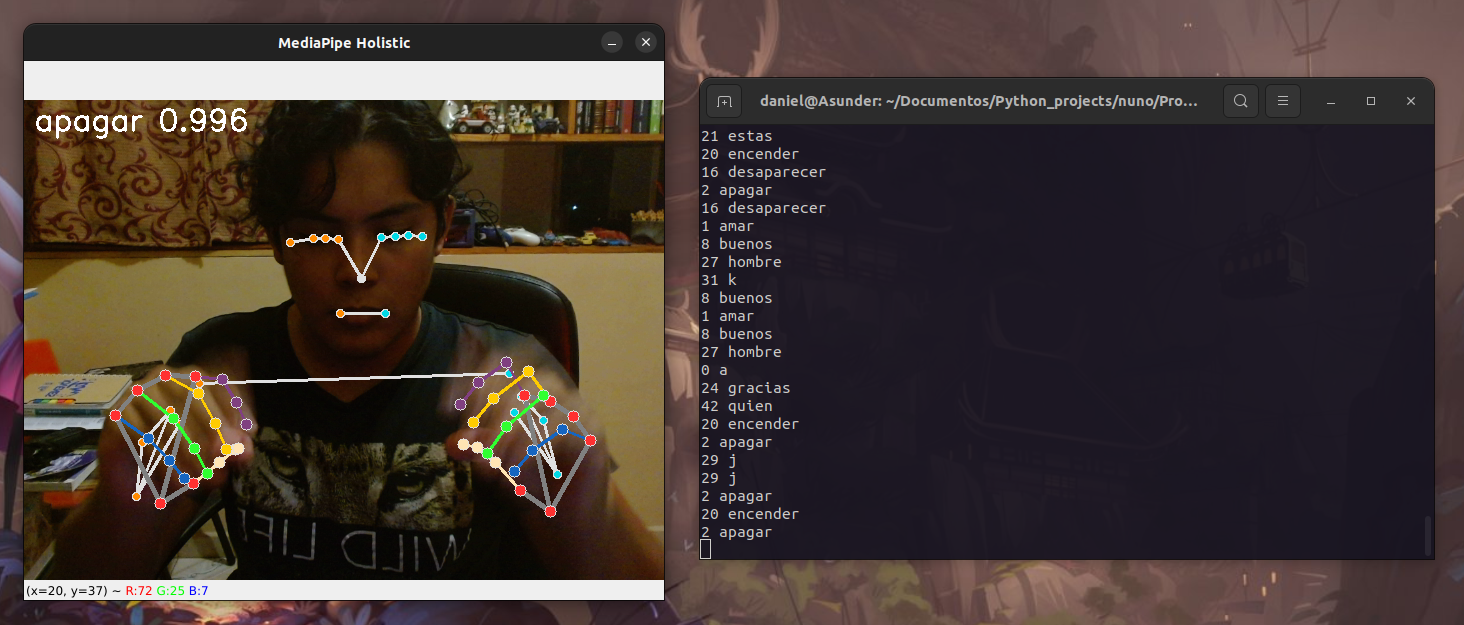
\includegraphics[width=0.95\linewidth]{img/08.png}}
\caption{Seña de la palabra "apagar"}
\label{fig:8}
\end{figure}

\begin{figure}[h]
\centering
{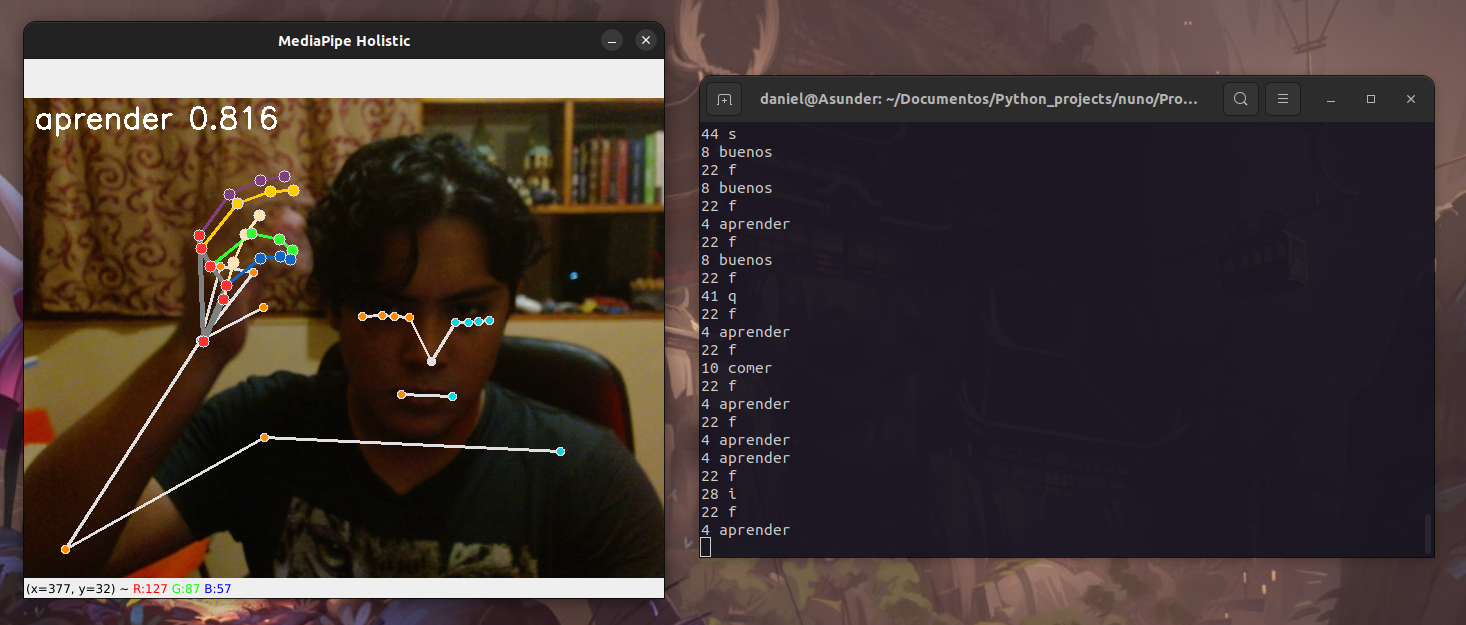
\includegraphics[width=0.95\linewidth]{img/09.png}}
\caption{Seña de la palabra "aprender"}
\label{fig:9}
\end{figure}

Como resultado final se obtiene un total de 22 pruebas realizadas e implementadas con éxito, estas pruebas pueden ser observadas en la figura \ref{fig:pruebas} donde se muestra una gran variedad de palabras para poner en ejecución en el programa de lenguaje de señas Mexicano, así mismo se anexan videos de retroalimentación para poder visualizar más a detalle cómo se realiza la prueba de manera correcta de acuerdo a especialistas en el tema:

\begin{figure}[h]
\centering
{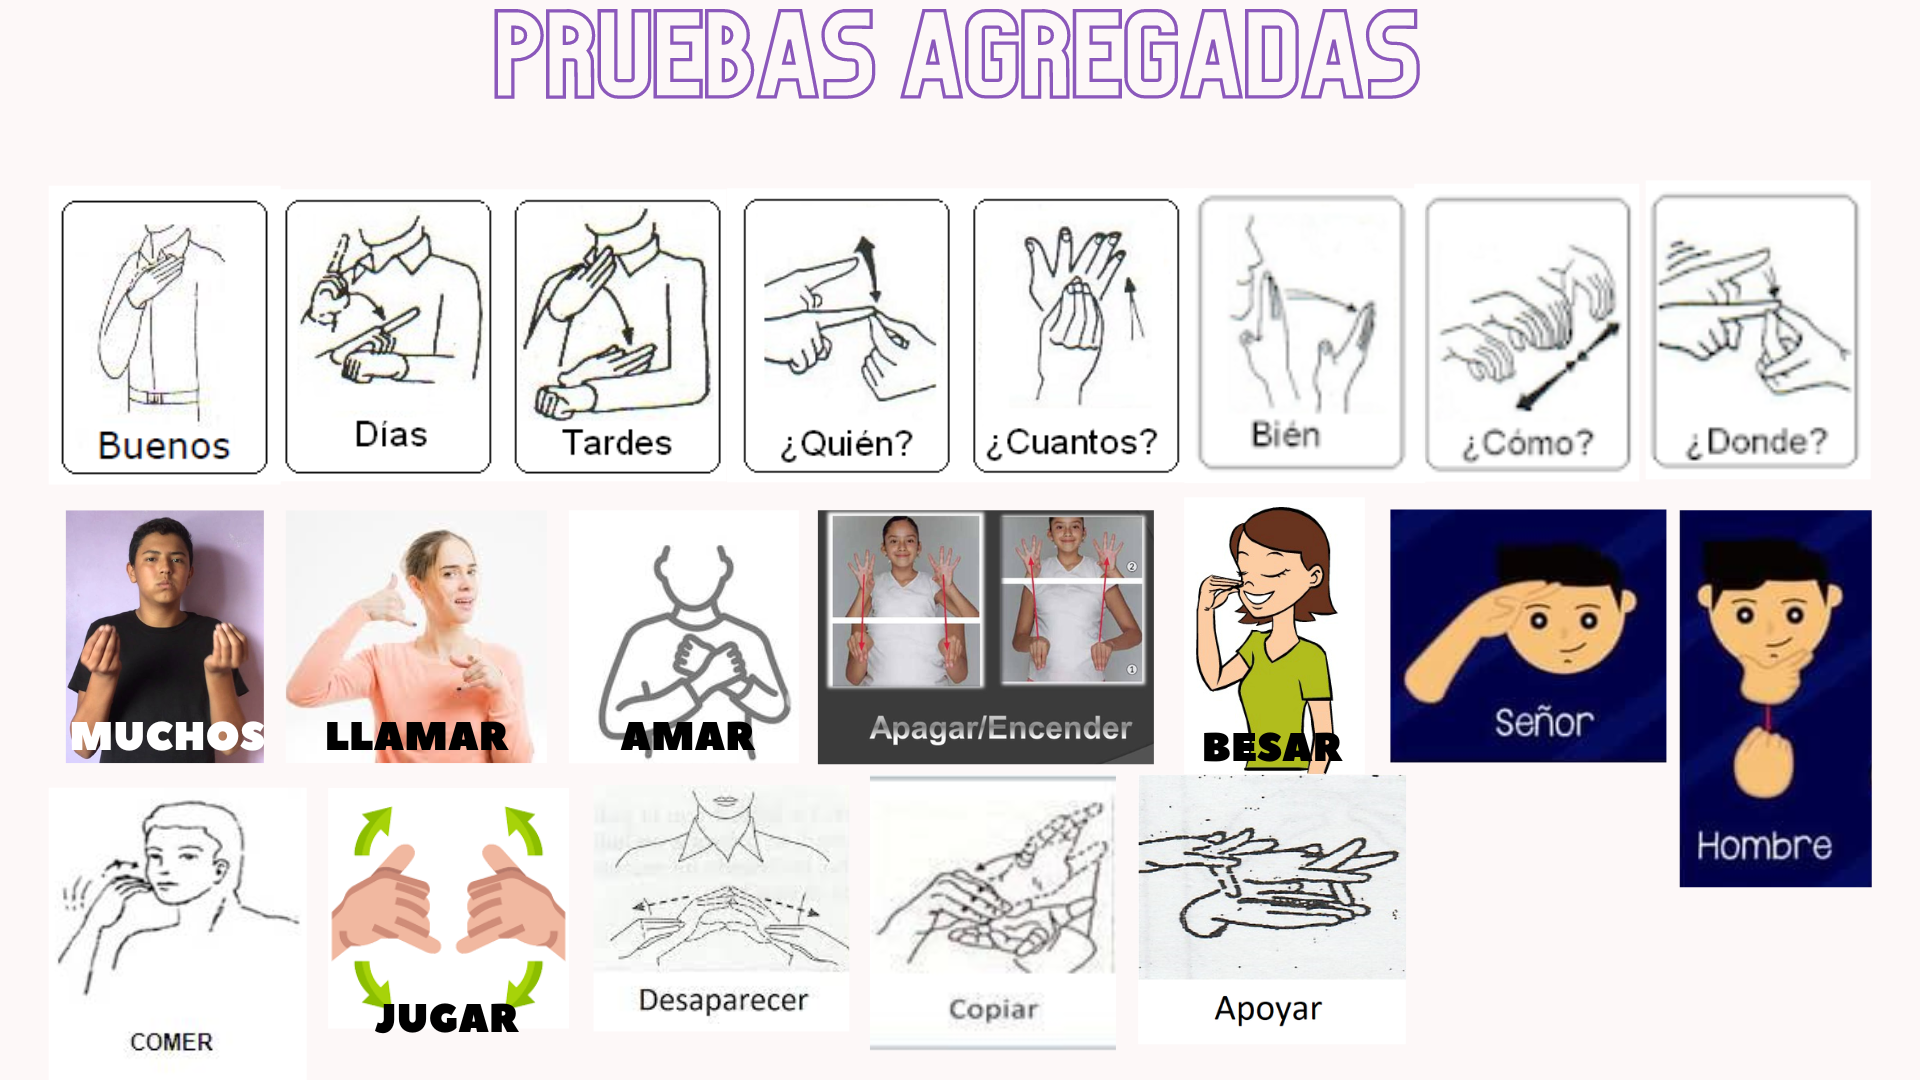
\includegraphics[width=0.95\linewidth]{img/Pruebas agregadas.png}}
    \caption{Pruebas desarrolladas}
\label{fig:pruebas}
\end{figure}

\begin{itemize}
    \item Para las pruebas de (buenos, días, tardes, muchos) ver el \href{https://www.youtube.com/shorts/NHADjfgkAjA}{video de YouTube} 

    \item Para las pruebas de (quien, como, donde, cuantos) ver el
    \href{https://www.youtube.com/watch?v=6XGl2R5JMyc }{video de YouTube} 

    \item Para las pruebas de (hombre, señor) vistas en la imagen de pruebas desarrolladas en la figura \ref{fig:pruebas}

    \item Para las pruebas de  (llamar, amar, encender, apagar, apoyar, besar, comer, desaparecer, copiar, jugar) ver el
    \href{https://www.youtube.com/watch?v=WXj9XSjwZcI}{video de YouTube} 

    \item Para las pruebas de (estas, bien) ver el \href{https://www.youtube.com/watch?v=8KVeaX35zLQ&t=180s }{video de YouTube}

\hfill \break
De acuerdo con los resultados de las pruebas realizadas, se han obtenido los siguientes parámetros:
\begin{table}[h]
\centering
\caption{Resultados de Señas}
\begin{tabular}{|c|c|c|}
\hline
\textbf{Seña} & \textbf{Aciertos} & \textbf{Fallos} \\
\hline
buenos & 19 & 1 \\
\hline
dias & 18 & 2 \\
\hline
tardes & 20 & 0 \\
\hline
quien & 16 & 4 \\
\hline
cuantos & 17 & 3 \\
\hline
bien & 19 & 1 \\
\hline
estas & 19 & 1 \\
\hline
como & 18 & 2 \\
\hline
donde & 19 & 1 \\
\hline
muchos & 15 & 5 \\
\hline
llamar & 17 & 3 \\
\hline
amar & 18 & 2 \\
\hline
apagar & 8 & 12 \\
\hline
encender & 20 & 0 \\
\hline
besar & 18 & 2 \\
\hline
senor & 19 & 1 \\
\hline
hombre & 20 & 0 \\
\hline
comer & 19 & 1 \\
\hline
jugar & 17 & 3 \\
\hline
desaparecer & 18 & 2 \\
\hline
copiar & 16 & 4 \\
\hline
apoyar & 19 & 1 \\
\hline
\end{tabular}
\end{table}
\end{itemize}

Con los datos previamente mencionados, se ha creado exitosamente la matriz de confusión.

\begin{table*}[h!]
\centering
\caption{Matriz de Confusión}
\resizebox{\textwidth}{!}{%
\begin{adjustbox}{angle=0}
\begin{tabular}{|c|c|c|c|c|c|c|c|c|c|c|c|c|c|c|c|c|c|c|c|c|c|c|}
\hline
\textbf{Seña} & \textbf{buenos} & \textbf{dias} & \textbf{tardes} & \textbf{quien} & \textbf{cuantos} & \textbf{bien} & \textbf{estas} & \textbf{como} & \textbf{donde} & \textbf{muchos} & \textbf{llamar} & \textbf{amar} & \textbf{apagar} & \textbf{encender} & \textbf{besar} & \textbf{senor} & \textbf{hombre} & \textbf{comer} & \textbf{jugar} & \textbf{desaparecer} & \textbf{copiar} & \textbf{apoyar} \\
\hline
\textbf{buenos} & 19 & 2 & 0 & 4 & 3 & 1 & 1 & 2 & 1 & 5 & 3 & 2 & 12 & 0 & 2 & 1 & 0 & 1 & 3 & 2 & 4 & 1 \\
\hline
\textbf{dias} & 1 & 18 & 0 & 4 & 3 & 1 & 1 & 2 & 1 & 5 & 3 & 2 & 12 & 0 & 2 & 1 & 0 & 1 & 3 & 2 & 4 & 1 \\
\hline
\textbf{tardes} & 1 & 2 & 20 & 4 & 3 & 1 & 1 & 2 & 1 & 5 & 3 & 2 & 12 & 0 & 2 & 1 & 0 & 1 & 3 & 2 & 4 & 1 \\
\hline
\textbf{quien} & 1 & 2 & 0 & 16 & 3 & 1 & 1 & 2 & 1 & 5 & 3 & 2 & 12 & 0 & 2 & 1 & 0 & 1 & 3 & 2 & 4 & 1 \\
\hline
\textbf{cuantos} & 1 & 2 & 0 & 4 & 17 & 1 & 1 & 2 & 1 & 5 & 3 & 2 & 12 & 0 & 2 & 1 & 0 & 1 & 3 & 2 & 4 & 1 \\
\hline
\textbf{bien} & 1 & 2 & 0 & 4 & 3 & 19 & 1 & 2 & 1 & 5 & 3 & 2 & 12 & 0 & 2 & 1 & 0 & 1 & 3 & 2 & 4 & 1 \\
\hline
\textbf{estas} & 1 & 2 & 0 & 4 & 3 & 1 & 19 & 2 & 1 & 5 & 3 & 2 & 12 & 0 & 2 & 1 & 0 & 1 & 3 & 2 & 4 & 1 \\
\hline
\textbf{como} & 1 & 2 & 0 & 4 & 3 & 1 & 1 & 18 & 1 & 5 & 3 & 2 & 12 & 0 & 2 & 1 & 0 & 1 & 3 & 2 & 4 & 1 \\
\hline
\textbf{donde} & 1 & 2 & 0 & 4 & 3 & 1 & 1 & 2 & 19 & 5 & 3 & 2 & 12 & 0 & 2 & 1 & 0 & 1 & 3 & 2 & 4 & 1 \\
\hline
\textbf{muchos} & 1 & 2 & 0 & 4 & 3 & 1 & 1 & 2 & 1 & 15 & 3 & 2 & 12 & 0 & 2 & 1 & 0 & 1 & 3 & 2 & 4 & 1 \\
\hline
\textbf{llamar} & 1 & 2 & 0 & 4 & 3 & 1 & 1 & 2 & 1 & 5 & 17 & 2 & 12 & 0 & 2 & 1 & 0 & 1 & 3 & 2 & 4 & 1 \\
\hline
\textbf{amar} & 1 & 2 & 0 & 4 & 3 & 1 & 1 & 2 & 1 & 5 & 3 & 18 & 12 & 0 & 2 & 1 & 0 & 1 & 3 & 2 & 4 & 1 \\
\hline
\textbf{apagar} & 1 & 2 & 0 & 4 & 3 & 1 & 1 & 2 & 1 & 5 & 3 & 2 & 8 & 0 & 2 & 1 & 0 & 1 & 3 & 2 & 4 & 1 \\
\hline
\textbf{encender} & 1 & 2 & 0 & 4 & 3 & 1 & 1 & 2 & 1 & 5 & 3 & 2 & 12 & 20 & 2 & 1 & 0 & 1 & 3 & 2 & 4 & 1 \\
\hline
\textbf{besar} & 1 & 2 & 0 & 4 & 3 & 1 & 1 & 2 & 1 & 5 & 3 & 2 & 12 & 0 & 18 & 1 & 0 & 1 & 3 & 2 & 4 & 1 \\
\hline
\textbf{senor} & 1 & 2 & 0 & 4 & 3 & 1 & 1 & 2 & 1 & 5 & 3 & 2 & 12 & 0 & 2 & 1 & 0 & 1 & 3 & 2 & 4 & 1 \\
\hline
\textbf{hombre} & 1 & 2 & 0 & 4 & 3 & 1 & 1 & 2 & 1 & 5 & 3 & 2 & 12 & 0 & 2 & 1 & 0 & 1 & 3 & 2 & 4 & 1 \\
\hline
\textbf{comer} & 1 & 2 & 0 & 4 & 3 & 1 & 1 & 2 & 1 & 5 & 3 & 2 & 12 & 0 & 2 & 1 & 0 & 1 & 3 & 2 & 4 & 1 \\
\hline
\textbf{jugar} & 1 & 2 & 0 & 4 & 3 & 1 & 1 & 2 & 1 & 5 & 3 & 2 & 12 & 0 & 2 & 1 & 0 & 1 & 3 & 2 & 4 & 1 \\
\hline
\textbf{desaparecer} & 1 & 2 & 0 & 4 & 3 & 1 & 1 & 2 & 1 & 5 & 3 & 2 & 12 & 0 & 2 & 1 & 0 & 1 & 3 & 2 & 4 & 1 \\
\hline
\textbf{copiar} & 1 & 2 & 0 & 4 & 3 & 1 & 1 & 2 & 1 & 5 & 3 & 2 & 12 & 0 & 2 & 1 & 0 & 1 & 3 & 2 & 4 & 1 \\
\hline
\textbf{apoyar} & 1 & 2 & 0 & 4 & 3 & 1 & 1 & 2 & 1 & 5 & 3 & 2 & 12 & 0 & 2 & 1 & 0 & 1 & 3 & 2 & 4 & 19 \\
\hline
\end{tabular}
\end{adjustbox}
}
\end{table*}



\section{Conclusión}
En conclusión, este proyecto ha demostrado ser un éxito al ampliar el repertorio de gestos previamente entrenados en el modelo de redes neuronales desarrollado en Python. La incorporación exitosa de nuevos gestos, palabras y letras del lenguaje de señas mexicano, junto con la capacidad de detectarlos en tiempo real a través de una cámara web, refuerza la versatilidad y adaptabilidad de las redes neuronales en la interpretación de señales visuales complejas.

La expansión de la base de datos de gestos ha permitido fortalecer la precisión y confiabilidad del modelo, mejorando su capacidad para reconocer una gama más amplia de expresiones del lenguaje de señas.

\addcontentsline{toc}{section}{Referencias} 
\printbibliography
%\balance



\end{document}

